\documentclass[xetex,mathserif,serif]{beamer}
\usepackage{polyglossia}
\setdefaultlanguage[babelshorthands=true]{russian}
\usepackage{listings}
\usepackage{tabu}

\useoutertheme{infolines}

\usepackage{fontspec}
\setmainfont{FreeSans}
\newfontfamily{\russianfonttt}{FreeSans}

\setbeamertemplate{blocks}[rounded][shadow=false]
\setbeamercolor*{block title example}{fg=green!50!black,bg=green!20}
\setbeamercolor*{block body example}{fg=black,bg=green!10}

\setbeamercolor*{block title alerted}{fg=red!50!black,bg=red!20}
\setbeamercolor*{block body alerted}{fg=black,bg=red!10}

\lstset{language=Caml,basicstyle=\small\normalfont,keywordstyle=\color{red},showstringspaces=false}

\title{Введение в F\#}
\author{Юрий Литвинов}
\date{19.02.2016г}

\begin{document}
	
	\frame{\titlepage}
	
	\section{Введение}
	
	\begin{frame}
		\frametitle{F\#}
		\begin{itemize}
			\item Типизированный функциональный язык для платформы .NET
			\item НЕ чисто функциональный (можно императивный стиль и ООП)
			\item Первый раз представлен публике в 2005 г.
			\item Создавался под влиянием OCaml (практически диалект OCaml под .NET)
			\item Использует .NET CLI
			\item Компилируемый и интерпретируемый
			\item Используется в промышленности, в отличие от многих чисто функциональных языков
		\end{itemize}
	\end{frame}

	\begin{frame}
		\frametitle{Что скачать и поставить}
		\begin{itemize}
			\item Под Windows --- Visual Studio, из коробки
			\item Под Linux --- Mono + MonoDevelop + F\# Language Binding, из репозиториев
			\item Прямо в браузере: http://www.tryfsharp.org/Learn
		\end{itemize}
	\end{frame}
	
	\begin{frame}[fragile]
		\frametitle{Пример программы}
		\begin{exampleblock}{F\#}
			\begin{lstlisting}[showstringspaces=false]
printfn "%s" "Hello, world"
            \end{lstlisting}
		\end{exampleblock}
\end{frame}
		
	\begin{frame}[fragile]
		\frametitle{Ещё пример}
		\begin{exampleblock}{F\#}
			\begin{lstlisting}
let rec factorial x =
    if x = 1 then 1 else x * factorial (x - 1)
            \end{lstlisting}
		\end{exampleblock}
\end{frame}
	
	\section{Let-определения}

	\begin{frame}[fragile]
		\frametitle{let-определение}
		\framesubtitle{Как жить без переменных}
		\begin{exampleblock}{F\#}
			\begin{lstlisting}
let x = 1
let x = 2
printfn "%d" x
           \end{lstlisting}
		\end{exampleblock}
		можно читать как
		\begin{exampleblock}{F\#}
			\begin{lstlisting}
let x = 1 in let x = 2 in printfn "%d" x
            \end{lstlisting}
		\end{exampleblock}
		и понимать как подстановку $\lambda$-терма
\end{frame}
		
	\begin{frame}[fragile]
		\frametitle{let-определение, функции}
		\begin{exampleblock}{F\#}
			\begin{lstlisting}
let powerOfFour x = 
    let xSquared = x * x
    xSquared * xSquared
            \end{lstlisting}
		\end{exampleblock}
		\begin{itemize}
			\item Позиционный синтаксис
			\begin{itemize}
				\item Отступы строго пробелами
				\item Не надо ";"
			\end{itemize}
			\item Нет особых синтаксических различий между переменной и функцией
			\item Не надо писать типы
			\item Не надо писать \textit{return}
		\end{itemize}
\end{frame}

	\begin{frame}[fragile]
		\frametitle{Вложенные let-определения}
		\begin{exampleblock}{F\#}
			\begin{lstlisting}
let powerOfFourPlusTwoTimesSix n =
    let n3 =
        let n1 = n * n
        let n2 = n1 * n1
        n2 + 2
    let n4 = n3 * 6
    n4
            \end{lstlisting}
		\end{exampleblock}
		\begin{itemize}
			\item \textit{n3} --- не функция!
			\item Компилятор отличает значения и функции по наличию аргументов
			\item Значение вычисляется, когда до \textit{let} <<доходит управление>>, 
					функция --- когда её вызовут. Хотя, конечно, функция --- тоже значение.
		\end{itemize}
\end{frame}
			
	\section{Типы}
			
	\begin{frame}[fragile]
		\frametitle{Типы}
		\begin{exampleblock}{F\#}
			\begin{lstlisting}
let rec f x =
    if x = 1 then 
        1 
    else 
        x * f (x - 1)
            \end{lstlisting}
		\end{exampleblock}

		\begin{alertblock}{F\# Interactive}
			\begin{lstlisting}
val f : x:int -> int
            \end{lstlisting}
        \end{alertblock}
        Каждое значение имеет тип, известный во время компиляции
\end{frame}
			
	\begin{frame}
		\frametitle{Элементарные типы}
		\begin{itemize}
			\item \textit{int}
			\item \textit{double}
			\item \textit{bool}
			\item \textit{string}
			\item ... (.NET)
			\item \textit{unit} --- тип из одного значения, (). Аналог void.
		\end{itemize}
	\end{frame}
	
	\begin{frame}[fragile]
		\frametitle{Таплы}
		\begin{exampleblock}{F\#}
			\begin{lstlisting}
let site1 = ("scholar.google.com", 10)
let site2 = ("citeseerx.ist.psu.edu", 5)
let site3 = ("scopus.com", 4)
let sites = (site1, site2, site3)

let url, relevance = site1
let site1, site2, site3 = sites
            \end{lstlisting}
		\end{exampleblock}
\end{frame}

	\begin{frame}[fragile]
		\frametitle{Лямбды}
		\begin{exampleblock}{F\#}
			\begin{lstlisting}
let primes = [2; 3; 5; 7]
let primeCubes = List.map (fun n -> n * n * n) primes
            \end{lstlisting}
		\end{exampleblock}
		\begin{alertblock}{F\# Interactive}
			\begin{lstlisting}
> primeCubes;;
val it : int list = [8; 27; 125; 343]
            \end{lstlisting}
		\end{alertblock}
		\begin{exampleblock}{F\#}
			\begin{lstlisting}
let f = fun x -> x * x
let n = f 4
            \end{lstlisting}
		\end{exampleblock}
\end{frame}

	\begin{frame}
		\frametitle{Списки}
		\begin{small}
			\begin{tabu} {| X[0.9 l p] | X[1 l p] | X[1 l p] |}
				\tabucline-
				Синтаксис                               & Описание                  & Пример                             \\
				\tabucline-
				\everyrow{\tabucline-}
				$[]$                                    & Пустой список             & $[]$                               \\
				$[expr; ...; expr]$                     & Список с элементами       & $[1; 2; 3]$                        \\
				$expr :: list$                          & cons, добавление в голову & $1 :: [2; 3]$                      \\
				$[expr\ ..\ expr]$                      & Промежуток целых чисел    & $[1 .. 10]$                        \\
				$[for\ x\ in\ list\ \rightarrow\ expr]$ & Генерированный список     & $[for\ x\ in\ 1..99\ \rightarrow\ x\ *\ x]$ \\					
				$list\ @\ list$                         & Конкатенация              & $[1; 2]\ @\ [3; 4]$                \\					
			\end{tabu}
		\end{small}
	\end{frame}

	\begin{frame}[fragile]
		\frametitle{Примеры работы со списками}
		\begin{exampleblock}{F\#}
			\begin{lstlisting}
let oddPrimes = [3; 5; 7; 11]
let morePrimes = [13; 17]
let primes = 2 :: (oddPrimes @ morePrimes)
\end{lstlisting}
		\end{exampleblock}
		\begin{exampleblock}{F\#}
			\begin{lstlisting}
let printFirst primes =
    match primes with
    | h :: t -> printfn "First prime in the list is %d" h
    | [] -> printfn "No primes found in the list"			
\end{lstlisting}
		\end{exampleblock}
\end{frame}

	\begin{frame}[fragile]
		\frametitle{Устройство списков}
		\begin{center}
			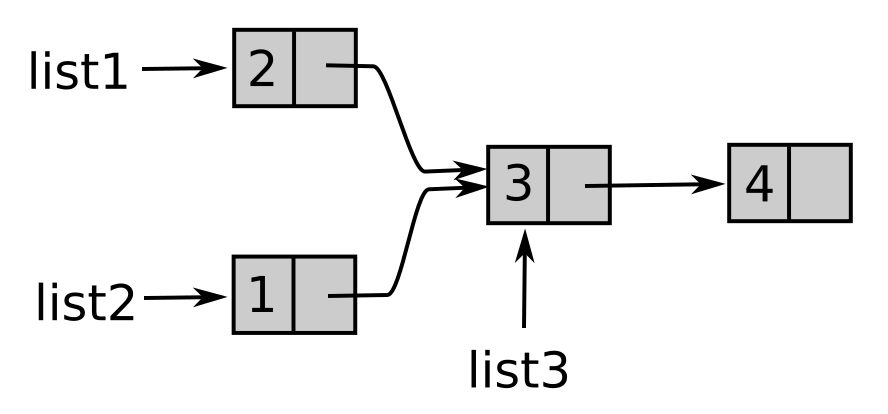
\includegraphics[width=0.4\textwidth]{lists.png}
		\end{center}
		\begin{exampleblock}{F\#}
			\begin{lstlisting}
let list3 = [3; 4]
let list1 = 2 :: list3
let list2 = 1 :: list3
            \end{lstlisting}
        \end{exampleblock}
		\begin{itemize}
			\item Списки немутабельны
			\item Cons-ячейки, указывающие друг на друга
			\item cons за константное время, @ --- за линейное
		\end{itemize}
\end{frame}

	\begin{frame}
		\frametitle{Операции над списками}
		\framesubtitle{Модуль Microsoft.FSharp.Collections.List}
		\begin{small}
			\begin{tabu} {| X[0.5 l p] | X[1 l p] | X[1 l p] | X[0.5 l p] |}
				\tabucline-
				Функция                & Описание                            & Пример                                              & Результат                        \\
				\tabucline-
				\everyrow{\tabucline-}
				List.length            & Длина списка                        & $List.length\ [1;2;3]$                              & $3$          \\
				List.nth               & n-ый элемент списка                 & $List.nth\ [1; 2; 3]\ 1$                            & $2$          \\
				List.init              & Генерирует список                   & $List.init\ 3 (fun\ i\ \rightarrow\ i * i)$         & $[0; 1; 4]$          \\
				List.head              & Голова списка                       & $List.head\ [1; 2; 3]$                              & $1$          \\
				List.tail              & Хвост списка                        & $List.tail\ [1; 2; 3]$                              & $[2; 3]$          \\
				List.map               & Применяет функцию ко всем элементам & $List.map\ (fun\ i\ \rightarrow\ i * i)\ [1; 2; 3]$ & $[1; 4; 9]$          \\
				List.filter            & Отбирает нужные элементы            & $List.filter\ (fun\ x\ \rightarrow\ x\ \%\ 2 <> 0)\ [1; 2; 3]$ & $[1; 3]$          \\
				List.fold              & "Свёртка"  & $List.fold\ (fun\ x\ acc\ \rightarrow\ acc * x)\ 1\ [1; 2; 3]$               & $6$          \\
				List.zip               & Делает из двух списков список пар   & $List.zip\ [1; 2]\ [3; 4]$                          & $[(1, 3); (2, 4)]$          \\
			\end{tabu}
		\end{small}
	\end{frame}
	
	\begin{frame}[fragile]
		\frametitle{Тип Option}
		Либо \textit{Some что-то}, либо \textit{None}, представляет возможное отсутствие значения.
		\begin{exampleblock}{F\#}
			\begin{lstlisting}
let people = [ ("Adam", None); ("Eve" , None);
    ("Cain", Some("Adam","Eve"));
    ("Abel", Some("Adam","Eve")) ]
            \end{lstlisting}
		\end{exampleblock}
		\begin{exampleblock}{F\#}
			\begin{lstlisting}
let showParents (name, parents) =
    match parents with
    | Some(dad, mum) -> 
        printfn "%s, father %s, mother %s" name dad mum
    | None -> printfn "%s has no parents!" name
            \end{lstlisting}
		\end{exampleblock}
\end{frame}

	\section{Функции}

	\begin{frame}[fragile]
		\frametitle{Рекурсия}
		\begin{exampleblock}{F\#}
			\begin{lstlisting}
let rec length l =
    match l with
    | [] -> 0
    | h :: t -> 1 + length t

let rec even n = (n = 0u) || odd(n - 1u)
and odd n = (n <> 0u) && even(n - 1u)			
            \end{lstlisting}
		\end{exampleblock}
\end{frame}

	\begin{frame}[fragile]
		\frametitle{Операторы $|>$ и $>>$}
		\framesubtitle{Forward pipeline и Композиция}
		\begin{exampleblock}{F\#}
			\begin{lstlisting}
let sumFirst3 ls = ls |> Seq.take 3 |> Seq.fold (+) 0
            \end{lstlisting}
        \end{exampleblock}
        или
		\begin{exampleblock}{F\#}
			\begin{lstlisting}
let sumFirst3 = Seq.take 3 >> Seq.fold (+) 0
            \end{lstlisting}
		\end{exampleblock}
\end{frame}

	\begin{frame}[fragile]
		\frametitle{Каррирование, частичное применение}
		\begin{exampleblock}{F\#}
			\begin{lstlisting}
let shift (dx, dy) (px, py) = (px + dx, py + dy)
let shiftRight = shift (1, 0)
let shiftUp = shift (0, 1)
let shiftLeft = shift (-1, 0)
let shiftDown = shift (0, -1)
            \end{lstlisting}
		\end{exampleblock}
		\begin{alertblock}{F\#}
			\begin{lstlisting}
> shiftDown (1, 1);;
val it : int * int = (1, 0)
            \end{lstlisting}
		\end{alertblock}
\end{frame}

	\begin{frame}[fragile]
		\frametitle{Использование библиотек .NET}
		\begin{exampleblock}{F\#}
			\begin{lstlisting}[basicstyle=\ttfamily\tiny]
open System.Windows.Forms

let form = new Form(Visible = false, TopMost = true, Text = "Welcome to F#")
let textB = new RichTextBox(Dock = DockStyle.Fill, Text = "Some text")
form.Controls.Add(textB)

open System.IO
open System.Net

/// Get the contents of the URL via a web request
let http(url: string) =
    let req = System.Net.WebRequest.Create(url)
    let resp = req.GetResponse()
    let stream = resp.GetResponseStream()
    let reader = new StreamReader(stream)
    let html = reader.ReadToEnd()
    resp.Close()
    html

textB.Text <- http("http://www.google.com")

form.ShowDialog () |> ignore
           \end{lstlisting}
       \end{exampleblock}
\end{frame}

	\begin{frame}
		\frametitle{Ограничения на домашку}
		Нельзя пользоваться:
		\begin{itemize}
			\item мутабельными переменными
			\item массивами
			\item циклами
			\item другими императивными возможностями языка
		\end{itemize}
	\end{frame}

\end{document}